Community detection\ignore{, also know as clustering,} is the problem of uncovering the underlying structure of complex networks, i.e., identifying groups of vertices that exhibit dense internal connections but sparse connections with the rest of the network, in an unsupervised manner. It is an NP-hard problem with numerous applications in domains such as drug discovery, protein annotation, topic discovery, anomaly detection, and criminal identification. Communities identified are intrinsic when based on network topology alone, and are disjoint when each vertex belongs to only one community \cite{com-gregory10}. One of the difficulties in the community detection problem is the lack of apriori knowledge on the number and size distribution of communities \cite{com-blondel08}. The \textit{Louvain} method \cite{com-blondel08} is a popular heuristic-based approach for community detection, with the modularity metric \cite{com-newman06} being used to measure the quality of communities identified.

In recent years, the collection of data and the relationships among them, represented as graphs, have reached unmatched levels. This has necessitated the design of efficient parallel algorithms for community detection on large networks. Existing studies on Louvain propose\ignore{a number of algorithmic} several optimizations \cite{com-rotta11, com-waltman13, com-gach14, com-traag15, com-lu15, com-ryu16, com-ozaki16, com-naim17, com-halappanavar17, com-ghosh18, com-traag19, com-zhang21, com-shi21, com-you22, com-aldabobi22} and parallelization techniques \cite{com-cheong13, com-wickramaarachchi14, com-lu15, com-zeng15, com-que15, com-naim17, com-fazlali17, com-halappanavar17, com-zeitz17, com-ghosh18, com-bhowmik19, com-gheibi20, com-shi21, com-bhowmick22}. Further, significant research effort has been focused on developing efficient parallel implementations of Louvain algorithm for multicore CPUs \cite{staudt2015engineering, staudt2016networkit, com-fazlali17, com-halappanavar17, qie2022isolate}, GPUs \cite{com-naim17}, CPU-GPU hybrids \cite{com-bhowmik19, com-mohammadi20}, multi-GPUs \cite{com-cheong13, hricik2020using, chou2022batched, com-gawande22}, and multi-node systems --- CPU only \cite{com-ghosh18, ghosh2018scalable, sattar2022scalable} / CPU-GPU hybrids \cite{com-bhowmick22}.

However, many of the aforementioned works concentrate on optimizing the local-moving phase of the Louvain algorithm, but do not address optimization for the aggregation phase of the algorithm, which emerges as a bottleneck after the local-moving phase has been optimized.\ignore{Some implementations also fail to adequately parallelize the algorithm.} These optimization techniques are also scattered over a number of papers, making it difficult for a reader to get a grip over them. Moreover, much attention has been directed towards GPU-based solutions. However, developing algorithms that efficiently utilize GPUs can be challenging both in terms of initial implementation and ongoing maintenance. Further, the soaring prices of GPUs present hurdles. The multicore/shared memory environment holds significance for community detection, owing to its energy efficiency and the prevalence of hardware with ample DRAM capacities. Through our implementation of the Louvain algorithm, we aim to underscore that CPUs remain adept at irregular computation\ignore{, especially for algorithms where workload diminishes progressively with each iteration}. Additionally, we show that achieving optimal performance necessitates a\ignore{heightened} focus on the\ignore{underlying} data structures\ignore{ rather than solely on algorithmic techniques, recognizing that algorithms are built upon these foundational structures}.

\ignore{Optimizing parallel community detection algorithms for modern hardware architectures can yield notable performance benefits and competitive advantages across applications. However, many of the current algorithms for community detection are challenging to parallelize due to their irregular and inherently sequential nature \cite{com-halappanavar17}, in addition to the complexities of handling concurrency, optimizing data access, reducing contention, minimizing load imbalance.}

In this\ignore{technical} report, we introduce our parallel multicore implementation of the Louvain algorithm\footnote{\url{https://github.com/puzzlef/louvain-communities-openmp}}. Our implementation employs asynchronous computation, utilizes parallel prefix sum and preallocated Compressed Sparse Row (CSR) data structures for identifying community vertices and storing the super-vertex graph during the aggregation phase, uses fast collision-free per-thread hash tables for the local-moving and aggregation phases, and incorporates an aggregation tolerance to avoid unnecessary aggregation phases. Additionally, we leverage established techniques such as threshold-scaling optimization, vertex pruning, limiting the number of iterations per pass, and OpenMP's \verb|dynamic| loop schedule. For each optimization, we determine optimal parameter settings, if there are any. To the best of our knowledge, our implementation represents the most efficient parallel Louvain algorithm implementation on multicore CPUs. We compare our implementation against other state-of-the-art implementations, including multi-core, multi-node, hybrid GPU, multi-GPU, and multi-node multi-GPU implementations, in Table \ref{tab:compare}. Both direct and indirect comparisons are provided, with details given in Sections \ref{sec:comparison} and \ref{sec:comparison-indirect} respectively.

\begin{table}[hbtp]
  \centering
  \caption{Speedup of our multicore implementation of Louvain algorithm compared to other state-of-the-art implementations. Direct comparisons are based on running the given implementation on our server, while indirect comparisons (denoted with a $*$, details given in Section \ref{sec:comparison-indirect}) involve comparing results obtained by the given implementation relative to a common reference (Grappolo).}
  \label{tab:compare}
  \begin{tabular}{|c|c||c|}
    \toprule
    \textbf{Louvain implementation} &
    \textbf{Published} &
    \textbf{Our Speedup} \\
    \midrule
    Grappolo \cite{com-halappanavar17} & 2017 & $22\times$ \\ \hline
    Vite \cite{ghosh2018scalable} & 2018 & $50\times$ \\ \hline
    NetworKit Louvain \cite{staudt2016networkit} & 2016 & $20\times$ \\ \hline
    DPLAL \cite{sattar2022scalable} & 2022 & $5472\times^*$ \\ \hline
    Qie et al. \cite{qie2022isolate} & 2022 & $273\times^*$ \\ \hline
    PLM \cite{staudt2015engineering} & 2015 & $48\times^*$ \\ \hline
    APLM \cite{com-fazlali17} & 2017 & $7.7\times^*$ \\ \hline
    Ghosh et al. (\ignore{8 }nodes) \cite{com-ghosh18} & 2018 & $5.9\times^*$ \\ \hline
    HyDetect (GPU) \cite{com-bhowmik19} & 2019 & $54\times^*$ \\ \hline
    Naim et al. (GPU) \cite{com-naim17} & 2017 & $9.8\times^*$ \\ \hline
    ACLM (GPU) \cite{com-mohammadi20} & 2020 & $6.0\times^*$ \\ \hline
    Chou and Ghosh (1 GPU) \cite{chou2022batched} & 2022 & $9.2\times^*$ \\ \hline
    cuVite (1 GPU) \cite{com-gawande22} & 2022 & $6.7\times^*$ \\ \hline
    cuGraph (1 GPU) \cite{hricik2020using} & 2020 & $4.8\times^*$ \\ \hline
    Cheong et al. (\ignore{16/24 }GPUs) \cite{com-cheong13} & 2013 & $8.3\times^*$ \\ \hline
    Bhowmick et al. (\ignore{8 }GPUs) \cite{com-bhowmick22} & 2022 & $4.9\times^*$ \\ \hline
  \bottomrule
  \end{tabular}
\end{table}





\ignore{\subsection{Our Contributions}}

\ignore{This report introduces GVE-Louvain, an optimized parallel implementation of Louvain\footnote{https://github.com/puzzlef/louvain-communities-openmp} for shared memory multicores. On a machine with two 16-core Intel Xeon Gold 6226R processors, GVE-Louvain outperforms Vite, Grappolo, and NetworKit Louvain by $50\times$, $22\times$, and $20\times$ respectively, achieving a processing rate of $560 M$ edges/s on a $3.8 B$ edge graph. With doubling of threads, GVE-Louvain exhibits an average performance scaling of $1.6\times$.}
%% NOTE: Vite is ghosh18scalable




%% - Use --- for a dash.
%% - Use ``camera-ready'' for quotes.
%% - Use {\itshape very} or \textit{very} for italicized text.
%% - Use \verb|acmart| or {\verb|acmart|} for mono-spaced text.
%% - Use \url{https://capitalizemytitle.com/} for URLs.
%% - Use {\bfseries Do not modify this document.} for important boldface details.
%% - Use \ref{fig:name} for referencing.

%% For a block of pre-formatted text: 
% \begin{verbatim}
%   \renewcommand{\shortauthors}{McCartney, et al.}
% \end{verbatim}

%% For a list of items:
% \begin{itemize}
% \item the ``ACM Reference Format'' text on the first page.
% \item the ``rights management'' text on the first page.
% \item the conference information in the page header(s).
% \end{itemize}

%% For a table:
% \begin{table}
%   \caption{Frequency of Special Characters}
%   \label{tab:freq}
%   \begin{tabular}{ccl}
%     \toprule
%     Non-English or Math&Frequency&Comments\\
%     \midrule
%     \O & 1 in 1,000& For Swedish names\\
%     $\pi$ & 1 in 5& Common in math\\
%     \$ & 4 in 5 & Used in business\\
%     $\Psi^2_1$ & 1 in 40,000& Unexplained usage\\
%   \bottomrule
% \end{tabular}
% \end{table}

%% For a full-width table:
% \begin{table*}
%   \caption{Some Typical Commands}
%   \label{tab:commands}
%   \begin{tabular}{ccl}
%     \toprule
%     Command &A Number & Comments\\
%     \midrule
%     \texttt{{\char'134}author} & 100& Author \\
%     \texttt{{\char'134}table}& 300 & For tables\\
%     \texttt{{\char'134}table*}& 400& For wider tables\\
%     \bottomrule
%   \end{tabular}
% \end{table*}


%% For inline math:
% \begin{math}
%   \lim_{n\rightarrow \infty}x=0
% \end{math},

%% For a numbered equation:
% \begin{equation}
%   \lim_{n\rightarrow \infty}x=0
% \end{equation}

%% For an unnumbered equation:
% \begin{displaymath}
%   \sum_{i=0}^{\infty} x + 1
% \end{displaymath}

%% For a figure:
% \begin{figure}[h]
%   \centering
%   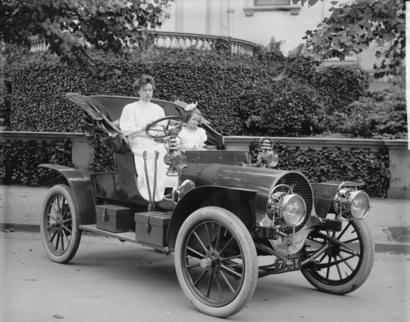
\includegraphics[width=\linewidth]{inc/sample-franklin}
%   \caption{1907 Franklin Model D roadster. Photograph by Harris \&
%     Ewing, Inc. [Public domain], via Wikimedia
%     Commons. (\url{https://goo.gl/VLCRBB}).}
%   \Description{A woman and a girl in white dresses sit in an open car.}
% \end{figure}

%% For a teaser figure.
% \begin{teaserfigure}
%   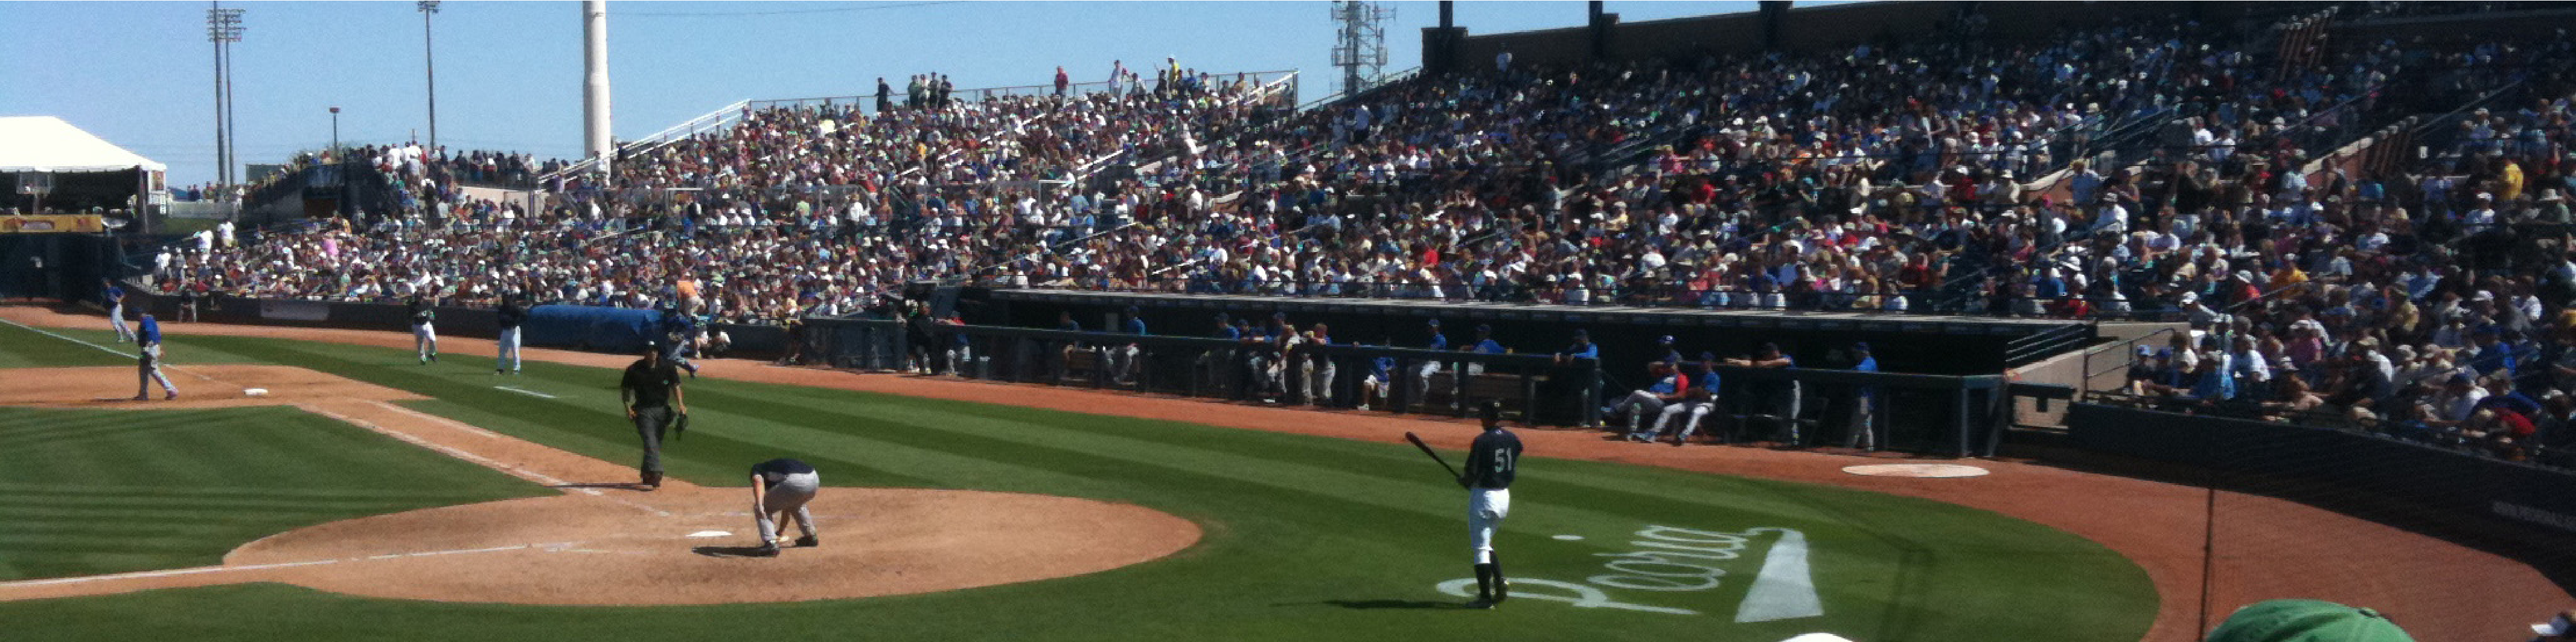
\includegraphics[width=\textwidth]{sampleteaser}
%   \caption{figure caption}
%   \Description{figure description}
% \end{teaserfigure}
